


\documentclass[14pt]{extreport}
\usepackage{gost}

\begin{document}

\pagestyle{empty}
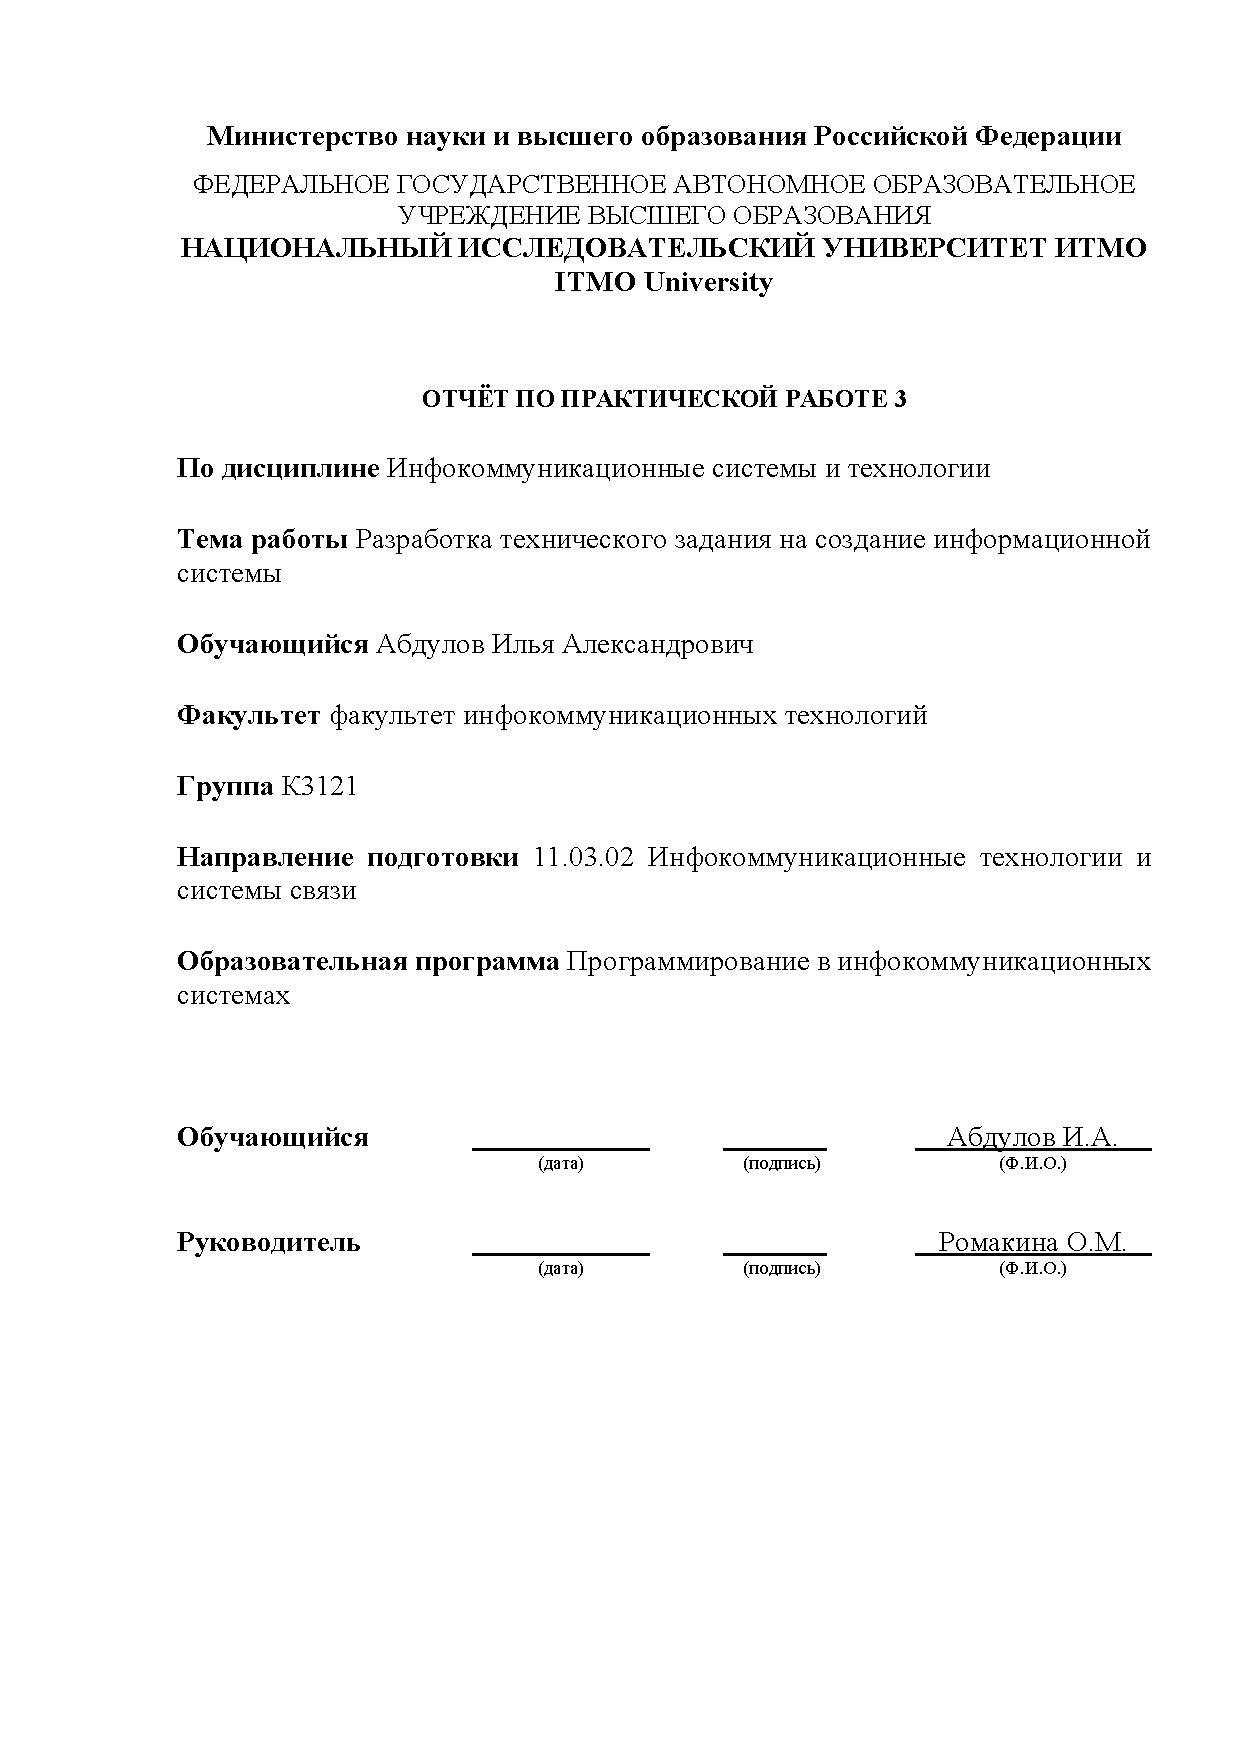
\includepdf{titulCourse.pdf}
\pagestyle{plain}

\tableofcontents

\intro

Практическая работа 8 является актуальной, потому что содержит техническое задание на разработку информационной системы.

Составление технического задания является важным этапом разработки любой информационной системы. Техническое задание находится в основании разработки ИС и помогает завершить проект в срок, минимизировать издержки, сократить время на разработку, разработать желаемый продукт.

Целью данной работы является составление технического задания на создание мобильного приложения.

\chapter{Общие сведения}

\section{Наименование работ}

Выполнение в 2022 году работ по созданию информационной системы для спортивного клуба по академической гребле "Rowing Club"\ университета ИТМО.

\section{Плановые сроки выполнения работ}

В течение 75 дней с даты заключения контракта в соответствии с календарным планом.

\section{Цели и задачи выполнения работ}

Основной целью выполнения работ является повышение уровня подготовки спортсменов по дисциплине гребля к межвузовским соревнованиям.

Выполняемые работы направлены на решение следующих задач:

\begin{itemize}
\item повышение уровня подготовки спортсменов к межвузовским соревнованием;
\item создание информационной системы клуба академической гребли "ITMO Rowing Club";
\item построение единой системы, содержащей всех гребцов университета ИТМО с их спортивными данными и показателями.
\end{itemize}

\section{Основные направления выполнения работ}

В рамках работ производится создание спортивного вузовского мобильного приложения, обеспечивающего процесс записи и анализа показателей спортсменов гребцов для отслеживания их прогресса.

\chapter{Общие требования к системе}

\section{Требования по сохранности информации при авариях}

Сохранность информации в развиваемой системе должна обеспечиваться при разрушении данных при механических и электронных сбоях и
отказах в работе компьютеров: на основе программных процедур
восстановления информации с использованием хранимых копий баз данных,
программных файлов системы, а также загружаемых файлов.

Система должна восстанавливаться при перезапуске аппаратных средств.

Для обеспечения сохранности информации в Системе должны быть
включены следующие функции:
\begin{itemize}
\item резервное копирование операционных систем, баз данных,
программных и загружаемых файлов;
\item восстановление данных в непротиворечивое состояние при
программно-аппаратных сбоях (отключение электрического питания, сбоях
операционной системы и других) вычислительно-операционной среды
функционирования;
\item	восстановление данных в непротиворечивое состояние при сбоях в
работе сетевого программного и аппаратного обеспечения.
\end{itemize}

\section{Требования к надежности}

Спроектированные архитектурные решения системы должны быть
устойчивы по отношению к программно-аппаратным ошибкам, отказам
технических и программных средств, с возможностью восстановления ее
работоспособности и целостности информационного содержимого при
возникновении ошибок и отказов.

\section{Требования к режимам функционирования}

Система должна иметь возможность функционировать в двух
режимах: штатном и режиме системного администрирования.

Штатный режим должен являться основным режимом
функционирования, обеспечивающим выполнение задач системы.

Режим системного администрирования должен являться технологическим
режимом и использоваться для сопровождения системы, в том числе –
изменения конфигурации, параметров работы, настроек, выполнения
регламентного обслуживания программно-технических средств. Кроме этого, в
режиме системного администрирования должны выполняться функции,
связанные с реконфигурацией, конвертированием и архивированием баз
данных системы. После возникновения отказа в каком-либо из компонентов
системы, режим должен обеспечивать перевод отказавших компонентов в
штатный режим функционирования после идентификации возникшего отказа и
устранения его причин.

\chapter{Создание информационной системы}

\section{Полное наименование системы}

Полное наименование: мобильное приложение Better Row.

Условное обозначение: Better Row.

\section{Цель работы}

Целью настоящей работы является создание мобильного приложения для развития спортивной деятельности в университете ИТМО, информационная система разрабатывается для клуба по академической гребле.

\section{Характеристика объекта автоматизации}

Объектами автоматизации являются процессы по управлению информационной системой, а также контроль эффективности выполнения программного обеспечения системы. 

Пользователями системы являются:
\begin{itemize}
\item руководство университета ИТМО;
\item руководство и представители гребного клуба университета;
\item участники гребного клуба университета;
\item персонал системы (администраторы).
\end{itemize}

Жалобы на эффективность работы информационной системы могут быть поданы:
\begin{itemize}
\item посредством портала системы;
\item по почте;
\item по мобильному телефону, указанным исполнителем.
\end{itemize}

\section{Требования к системе в целом}

Информационная система должна:
\begin{itemize}
\item упростить отслеживание тренировок;
\item сохранять записи о результатах тренировок;
\item отслеживать спортивный прогресс;
\item создавать аналитику по результатам тренировок.
\end{itemize}

\section{Требования к функциональной части системы}

Мобильное приложение Better Row должно состоять из:
\begin{itemize}
\item главного раздела, откуда осуществляется переход к основным подразделам приложения;
\item подраздела результатов и статистики, где отображаются добавленные тренировки по датам, и где можно добавить данные о новой тренировке;
\item подраздела расписания, где отображаются даты тренировок спортивного клуба;
\item подраздела настроек приложения, содержащего справочную и статистическую
информацию о приложении;
\item ЛК тренера или другого руководящего лица, обеспечивающий просмотр информации о результатах и прогрессе спортсменов;
\item ЛК спортсмена, обеспечивающий просмотр своих персональных данных.
\end{itemize}

Портал системы должен обеспечивать спортсмену:
\begin{itemize}
\item возможность внесения данных и показателей тренировки;
\item возможность сохранить результаты тренировки;
\item возможность удалить запись тренировки;
\item возможность просмотреть статистику тренировок;
\item возможность просмотреть прогресс тренировок. 
\end{itemize}

Портал системы должен обеспечивать руководству:
\begin{itemize}
\item возможность просмотреть список всех спортсменов в клубе;
\item возможность просмотреть статистику тренировок выбранного спортсмена;
\item возможность просмотреть прогресс спортсмена;
\item возможность удалить выбранного спортсмена из базы данных спортсменов.
\end{itemize}

Интерактивная форма внесения результатов тренировки должна обеспечивать внесение следующей информации:
\begin{itemize}
\item дистанция заплыва;
\item время заплыва;
\item темп заплыва;
\item пульс спортсмена.
\end{itemize}

Полученная информация о результате тренировки спортсмена должна размещаться в соответствующем подразделе результатов и статистики после прохождения формально-логической проверки автоматически сразу после поступления информации в систему. Автоматизированная формально-логическая проверка должна предусматривать проверку правильности заполнения интерактивных форм и полей ввода данных. В случае отрицательного результата проверки информация не должна вноситься в базу данных, лицо,
представившее информацию в систему, должно извещаться об этом
посредством системы и ему должна быть предоставлена возможность повторно
представить информацию в систему для внесения в базу данных с учетом
необходимых исправлений.

Система должна обеспечивать оперативное хранение записей тренировок спортсменов в течении 3 (трех) лет с момента их размещения в системе. По истечении указанного срока хранения информации о показателях тренировок спортсменов средствами СУБД предоставляет возможность выполнить её архивирование с возможностью доступа к ней администраторам системы.

В системе должна быть обеспечена возможность для руководства гребного клуба автоматической
выгрузки во внешнюю информационную среду информации по тренировкам спортсменов из мобильного приложения в виде электронной таблицы для удобной работы с большим количеством результатов и создания общепринятой отчетности.

\section{Требования к видам обеспечения}

\subsection{Требования, предъявляемые к математическому обеспечению}

Специальных требований к математическому обеспечению не
предъявляется. Специальные алгоритмы должны быть разработаны на стадии
технического проектирования.

\subsection{Требования, предъявляемые к информационному обеспечению}

Требования к информационному обеспечению определяются
функциональностью системы.

\subsection{Требования, предъявляемые к программному обеспечению}

Графический пользовательский интерфейс должен быть реализован как
мобильное приложение, используемое пользователями через мобильные устройства на операционной системе IOS, Android, ChromeOS версий, официально поддерживаемых производителями.

Макеты визуализации и дизайна форм системы должны быть разработаны и
представлены на этапе технического проектирования.

\subsection{Требования к организационному обеспечению}

В ходе выполнения работ в рамках данного технического задания должна
быть создана рабочая группа по управлению ходом работ, в состав которой
должны входить представители гребного клуба и исполнителя. Регламент взаимодействия представителей должен определяться в рабочем порядке.

\subsection{Проведение испытаний}

Испытания должны осуществляться в соответствии с этапами работ,
определенными в календарном плане, являющимся приложением к настоящему
техническому заданию, и оформляться в соответствии с требованиями,
приведенными в разделе «Требования к документированию» настоящего
документа.

Для системы должны быть проведены следующие работы:
\begin{itemize}
\item предварительные комплексные испытания;
\item опытная эксплуатация;
\item приемочные испытания.
\end{itemize}

Испытания должны проводиться комиссией, состоящей из
уполномоченных представителей сторон приема и исполнения работ.

Испытания должны проводиться с учетом требований ГОСТ 34.603-92
«Виды испытаний автоматизированных систем».

Проверка выполнения требований функционального назначения системы
должна осуществляться на заданном в качестве контрольного примера наборе
данных в пределах функций системы, указанных в настоящем документе, а
также уточняющих его технических требованиях к отдельным компонентам
системы, разработанных на этапе технического проектирования.

При обнаружении дефектов испытываемого программного обеспечения
список дефектов фиксируется, после чего комиссией утверждается срок
исправления дефектов и дата повторного проведения испытаний.

\chapter{Требования к результатам работ}

\section{Разработка прикладного программного обеспечения}

В ходе разработки прикладного программного обеспечения должны быть
выполнены следующие работы:
\begin{itemize}
\item разработка прикладного программного обеспечения согласно
требованиям настоящего технического задания;
\item установка и настройка прикладного программного обеспечения на
подготовленные технические средства, с установленным и настроенным
системным программным обеспечением. Технические средства для
демонстрации системы предоставляются исполнителем;
\item оформление исходных текстов прикладного программного обеспечения
и программной документации согласно требованиям настоящего
технического задания.
\end{itemize}

\section{Требования к составу и содержанию работ по подготовке объекта автоматизации к вводу системы в действие}

Система при вводе её в эксплуатацию должна пройти предварительные
комплексные испытания, опытную эксплуатацию и приемочные испытания.

Приемочным испытаниям системы должна предшествовать ее опытная
эксплуатация.

Исполнитель должен обеспечить функционирование системы в период
опытной эксплуатации на мощностях, определяемых гребным клубом.

В ходе подготовки объекта автоматизации к вводу системы в действие
должна быть произведена инсталляция общесистемного и прикладного программного
обеспечения. Инсталляция прикладного программного обеспечения должна
осуществляться в соответствии с руководством системного администратора со стороны исполнителя.

\chapter{Требования к документированию}

\section{Требования к оформлению}

Отчетная документация должна прилагаться в бумажном и электронном
виде (на оптическом CD или DVD или USB носителе) на русском языке.

Вспомогательная документация (не указанная в качестве непосредственного
результата работ) передается только в электронном виде.

Для каждого этапа должен быть представлен краткий отчет в форме
презентации.

\section{Проектная и рабочая документация}

Проектная и рабочая документация должна разрабатываться с учетом
требований комплекса государственных стандартов «Информационная
технология. Комплекс стандартов на автоматизированные системы»:
\begin{itemize}
\item ГОСТ 34.601-90 «Автоматизированные системы. Стадии создания»;
\item ГОСТ 34.003-90 «Автоматизированные системы. Термины и
определения»;
\item ГОСТ 34.602-89 «Техническое задание на создание
автоматизированной системы»;
\item ГОСТ 34.201-89 «Виды, комплектность и обозначение документов при
создании автоматизированных систем»;
\item ГОСТ 34.603-92 «Виды испытаний автоматизированных систем»;
\item РД 50-34.698-90 «Автоматизированные системы. Требования к
содержанию документов»;
\item ГОСТ 19.301-79 «Программа и методика испытаний. Требования к
содержанию и оформлению»;
\item ГОСТ 2.601-2006 «ЕСКД. Эксплуатационные документы»;
\item ГОСТ 2.106-96 «ЕСКД. Текстовые документы» (с изменениями от 22
июня 2006 года);
\item ГОСТ 2.120-73 «ЕСКД. Технический проект» (с изменениями от 22
июня 2006 года).
\end{itemize}

\section{Исходные тексты и программная документация}

Для каждой разрабатываемой системы должны быть представлены в
электронном виде (на оптическом CD или DVD или USB носителе):
\begin{itemize}
\item исходные тексты прикладного программного обеспечения, включая
контрольные суммы для каждого файла по алгоритму MD5;
\item инструкция по сборке из исходных текстов рабочего прикладного
программного обеспечения;
\item исполняемые файлы (где применимо), включая контрольные суммы
для каждого файла по алгоритму MD5;
\item описание программных средств, содержащее сведения об их
логической структуре и среде функционирования, а также описание методов,
приемов и правил эксплуатации технологических средств, используемых при
их создании;
\item описание применения, содержащее сведения о назначении
программных средств, области применения, применяемых методах, классе
решаемых задач, ограничениях при применении, минимальной конфигурации
технических средств, среде функционирования и порядке работы.
\end{itemize}

\section{Требования к оформлению документации по испытаниям системы}

Испытания развиваемой/создаваемой системы должны проводиться с
учетом требований ГОСТ 34.603-92 «Виды испытаний автоматизированных
систем».

\chapter{Источники разработки технического задания}

\section{Источники разработки}

Исходными документами для разработки данного технического задания и автоматизированной системы являются: материалы аналитического проектного исследования объекта автоматизации, действующие законодательные и нормативные правовые акты, в рамках которых функционирует объект автоматизации, нормативно-техническая документация, ГОСТ 34.602-89, образцы рабочих документов, полученных в процессе исследования, информационные материалы и проектная документация на аналогичные автоматизированные системы.

\conclusions

Цель работы была достигнута. Было составлено техническое задание на создание мобильного приложения.

Составление технического задания на мобильное приложение является важным этапом разработки информационной системы. Правильно составленное ТЗ помогает:
\begin{enumerate}
\item увеличить шансы создать продукт, соответствующий задачам бизнеса;
\item подготовить точный прогноз относительно сроков и стоимости разработки;
\item избежать конфликтов между исполнителем и заказчиком из-за разного понимания задач и методов решения;
\item сократить риски изменений проекта из-за нечетко прописанных требований.
\end{enumerate}

\newpage
\begin{thebibliography}{99}

\bibitem{bib1}Примеры технических заданий, составленных для аналогичных проектов — URL: \url{https://drive.google.com/drive/folders/1XbbDN72k7BuWoNRZJvKtHSEjfunnMn7w} (дата обращения 14.12.2022).

\bibitem{bib2}Комплекс стандартов на создание технического задания для автоматизированных систем ГОСТ 34.602-89 — URL: \url{https://drive.google.com/drive/folders/1L2nVVB2jm_JoFxdwLdpV8nnh6FVtEjEo} (дата обращения 14.12.2022).

\bibitem{bib3}Интернет-статья "Как написать ТЗ для мобильного приложения?"\ — URL: \url{https://sibdev.pro/blog/articles/kak-napisat-tz-dlya-mobilnogo-prilozheniya} (дата обращения 12.12.2022).

\bibitem{bib4}Интернет-статья "Разработка мобильного приложения: как написать техническое задание?"\ — URL: \url{https://sandev.ru/razrabotka-mobilnogo-prilozheniya-kak-napisat-tehnicheskoe-zadanie/} (дата обращения 14.12.2022).

\bibitem{bib5}Видео-лекция "ГОСТ 34 в современной разработке"\  — URL: \url{https://www.youtube.com/watch?v=Cb7oyeIjWZ8} (дата обращения 14.12.2022).
	
\end{thebibliography}

\end{document}
